\chapter{Diseño e implementación} % Main chapter title

\label{Chapter3} % Change X to a consecutive number; for referencing this chapter elsewhere, use \ref{ChapterX}

ESCRIBIR INTRODUCCION AL CAPITULO 3

%----------------------------------------------------------------------------------------
%	ADQUISICION DE DATOS
%----------------------------------------------------------------------------------------
\section{Adquisición de datos}
 
\newcommand{\myhash}{\raisebox{\depth}{\#}}

Para llevar a cabo el presente trabajo, se emplearon datos proporcionados por el servicio 
de cardiología e hipertensión del Hospital Alemán. La figura \ref{fig:adquisicion_datos} 
exhibe un diagrama en bloques que ilustra la etapa de adquisición de datos utilizada. 
Es importante destacar que se utilizaron dos conjuntos de datos diferentes. 

\begin{figure}[ht]
	\centering
	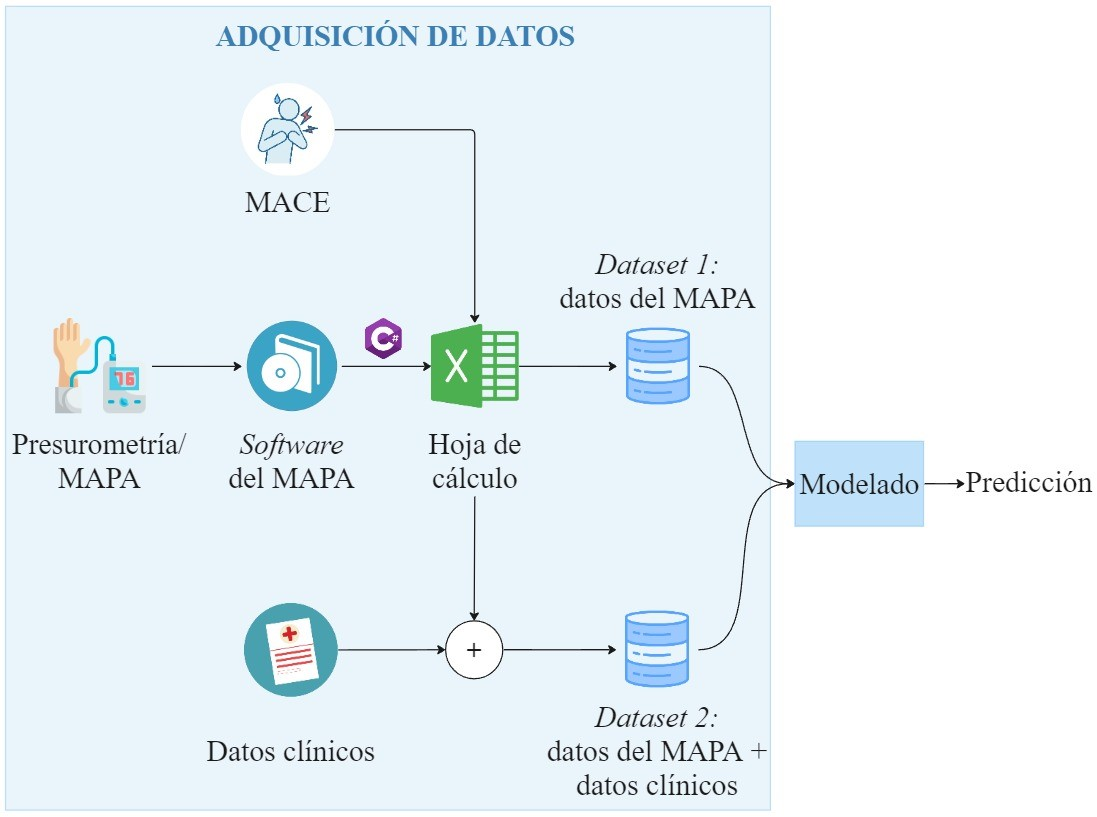
\includegraphics[width=\textwidth]{./Figures/adquisicion_datos2.jpg}
	\caption{Representación esquemática de las etapa de adquisición de datos.}\label{fig:adquisicion_datos}
\end{figure}

El primer \emph{dataset} se compone exclusivamente de información recopilada de las 
presurometrías realizadas a los pacientes hipertensos a partir del año 2013. Luego 
de realizar un MAPA, los datos se almacenan en un \emph{software} especializado de 
los presurómetros. Posteriormente, se extraen utilizando un programa desarrollado 
en C\myhash para ser registrados en una planilla de cálculo. Sumado a esto, se incluyó 
la variable a predecir (MACE) para cada paciente mediante un análisis exhaustivo 
de su historial clínico. Especificamente, se registró la ocurrencia de 
un accidente cerebrovascular no fatal, infarto agudo de miocardio, insuficiencia 
cardíaca, insuficiencia renal crónica o muerte. En caso de que correspondiera, también 
se incluyó la fecha correspondiente en la que tuvo lugar el evento.

Por otro lado, el segundo conjunto de datos contiene información adicional obtenida 
del historial clínico de cada paciente. Estos datos clínicos se agregan a la misma 
hoja de cálculo mencionada anteriormente, complementando así la información proveniente 
de las presurometrías.

El objetivo de utilizar dos \emph{datasets} es evaluar la calidad de los datos de 
las presurometrías para generar inferencias de manera independiente. En otras palabras, 
se buscó determinar en qué medida los datos del MAPA pueden ser utilizados por sí solos 
para obtener predicciones significativas y precisas de MACE. Al mismo tiempo, se procuró 
evaluar si la incorporación de información clínica contribuye a un mejor desempeño del 
modelo en términos de tasa de falsos negativos, AUC y otras métricas relevantes.


%----------------------------------------------------------------------------------------
% 3.1.1 Descripción del conjunto de datos

\subsection{Descripción del conjunto de datos}

El primer conjunto de datos comprende las variables derivadas del MAPA, junto con 
el valor de MACE y la fecha del evento asociado. A continuación, se brinda una 
descripción detallada de las variables provenientes de las presurometrías: 

\begin{itemize}
  \item Fechaest: corresponde a la fecha en la cual se realizó la presurometría.
  \item PASm24: representa la presión arterial sistólica media durante todo el MAPA.
	\item PADm24: representa la presión arterial diastólica media durante todo el MAPA.
  \item FCm24: representa la frecuencia cardíaca media durante todo el MAPA.
  \item PAMm24: representa la presión arterial media durante todo el MAPA.
  \item PPm24: representa la presión de pulso media durante todo el MAPA.
  \item PASsd24: indica el desvío estándar de la presión arterial sistólica media durante todo el MAPA. 
  \item PADsd24: indica el desvío estándar de la presión arterial diastólica media durante todo el MAPA.
  \item FCsd24:  indica el desvío estándar de la frecuencia cardíaca media durante todo el MAPA.
  \item PAMsd24: indica el desvío estándar de la presión arterial media durante todo el MAPA.
  \item PPsd24: indica el desvío estándar de la presión de pulso media durante todo el MAPA.
  \item PASmDIA: representa la presión arterial sistólica media diurna.
  \item PADmDIA: representa la presión arterial diastólica media diurna.
  \item FCmDIA: representa la frecuencia cardíaca media diurna.
  \item PAMmDIA: representa la presión arterial media diurna.
  \item PPmDIA: representa la presión de pulso media diurna.
  \item htaloadsbpDIA: se refiere al porcentaje de lecturas de la presión arterial sistólica que exceden el valor de referencia de 135 mmHg durante el día.
  \item htaloaddbpDIA: se refiere al porcentaje de lecturas de la presión arterial diastólica que exceden el valor de referencia de 85 mmHg durante el día.
  \item HTAdia01: se utiliza para determinar si un paciente presenta hipertensión diurna (HTAdia01 = 1) o normotensión diurna (HTAdia01 = 0). Se considera hipertensión diurna cuando la presión arterial sistólica es superior a 135 mmHg y la presión arterial diastólica es superior a 85 mmHg durante el día, mientras que se define como normotensión diurna cuando no se cumplen estos criterios.
  \item PASmNOCHE: representa la presión arterial sistólica media nocturna.
  \item PADmNOCHE: representa la presión arterial diastólica media nocturna.
  \item FCmNOCHE: representa la frecuencia cardíaca media nocturna.
	\item PAMmNOCHE: representa la presión arterial media nocturna.
	\item PPmNOCHE: representa la presión de pulso media nocturna.
  \item htaloadsbpNOCHE: representa el porcentaje de lecturas de la presión arterial sistólica que exceden el valor de referencia de 125 mmHg durante la noche.
  \item htaloaddbpNOCHE: se refiere al porcentaje de lecturas de la presión arterial diastólica que exceden el valor de referencia de 70 mmHg durante la noche.
  \item HTAnoche01: se define como hipertensión nocturna (HTAnoche01 = 1) cuando la presión arterial sistólica es superior a 120 mmHg y la presión arterial diastólica es superior a 70 mmHg durante la noche. En caso contrario, se considera normotensión nocturna (HTAnoche01 = 0).
  \item Nondipper01: se utiliza para clasificar a los pacientes en función de la disminución de la presión arterial durante la noche. Cuando la presión arterial no disminuye en un 10\% durante la noche, se considera un indicador de alto riesgo cardiovascular y se denominan \emph{non-dippers} (Nondipper01 = 1). Por otro lado, aquellos pacientes cuya presión arterial disminuye en un 10\% durante la noche se denominan \emph{dippers} (Nondipper01 = 0).
\end{itemize}


El segundo conjunto de datos, por su parte, incluye todas las variables mencionadas anteriormente, junto con
9 variables adicionales extraídas del historial clínico de cada paciente. Estas incluyen:

\begin{itemize}
  \item Talla: se refiere a la medida de la longitud del cuerpo de una persona y se expresa en centímetros.
  \item Peso: se refiere a la medida de la masa corporal del paciente expresada en kilogramos.
  \item IMC: el índice de masa corporal (IMC) es una medida utilizada para evaluar la relación entre el peso y la estatura de una persona. Se calcula dividiendo el peso en kilogramos por el cuadrado de la estatura en metros.
  \item Edad: representa el tiempo transcurrido desde el nacimiento de un individuo, medido en años.
  \item Sexo: indica si el paciente es hombre (Sexo = 0) o mujer (Sexo = 1).
  \item DBT: indica la presencia (DBT = 1) o ausencia (DBT = 0) de diabetes en un paciente, una enfermedad metabólica crónica caracterizada por niveles elevados de glucosa en sangre.
  \item Tabaquismo: indica si un paciente tiene adicción a la nicotina (Tabaquismo = 1) o no presenta dicha adicción (Tabaquismo = 0).
  \item Dislipemia: señala la presencia (Dislipemia = 1) o ausencia (Dislipemia = 0) de una alteración en los niveles de lípidos en sangre en un paciente.
  \item HVI: indica la presencia (HVI = 1) o ausencia (HVI = 0) de un engrosamiento de la pared del ventrículo izquierdo como consecuencia de la hipertensión en el paciente.
\end{itemize}

%------------------------------------------------------------------------
%	ANALISIS EXPLORATORIO DE DATOS
%----------------------------------------------------------------------------------------
\section{Análisis exploratorio de datos}
 